\section{Métodos e domínio de análise}

A análise compara a contribuição preditiva incremental de informações textuais para a popularidade Spotify observada no snapshot da fonte. O domínio analítico contém 77.535 faixas com letras aceitas, provenientes da amostra estratificada original de 200.000 faixas. A disponibilidade das letras não assegura representatividade do catálogo ou de todas as músicas com letras; por isso, as conclusões se referem ao domínio observado.


As quatro configurações usam as mesmas observações: Baseline, com 15 campos de metadados e acústicas; Tradicional, acrescentando 21 descritores lexicais e estruturais; Profundo, acrescentando embeddings multilingues de 384 dimensões; e Combinado, reunindo as duas representações textuais. Descritores e embeddings derivam do mesmo texto aceito padronizado. O encoder intfloat/multilingual-e5-small permaneceu congelado, sem ajuste pela resposta.


A avaliação empregou validação cruzada aninhada agrupada, com cinco folds externos e três internos. Os 21.893 componentes operacionais, maior com 186 faixas, unem artistas, participações explícitas, composições e textos iguais segundo regras documentadas. Cada faixa recebeu uma previsão externa de ajuste que não utilizou seu componente. Chaves operacionais não são identificadores universais.


A família Ridge foi mantida entre blocos, com alpha em 0,1; 1; 10; 100; 1.000; 10.000 e seleção por MAE interno não ponderado. Imputação, escala e categorias foram aprendidas apenas em cada treino. Foram executados 360 ajustes internos, 20 refits externos e dez referências média/mediana. Não houve PCA, ajuste do encoder, clipping ou expansão da grade após resultados externos. Esse cuidado distingue seleção e avaliação, conforme Cawley e Talbot (2010).


O ajuste e as métricas principais atribuem pesos iguais às faixas. MAE é a métrica primária, com RMSE e R² complementares calculados sobre previsões externas reunidas. A sensibilidade usa os pesos amostrais originais apenas no MAE, nas mesmas previsões. Esses pesos não corrigem automaticamente a disponibilidade textual. O teste histórico v0.6 já havia sido aberto em 14/10/2026; nova CV não restaura confirmação independente.


\FloatBarrier

\clearpage

\section{Resultados globais e sensibilidade aos pesos}

O Combinado apresentou o menor MAE observado: 8,1151, frente a 8,3525 no Baseline. A redução foi de 0,2374 ponto, ou 2,842\%. Com pesos originais, a redução relativa foi de 2,781\%, mantendo a ordenação dos quatro blocos.


O Profundo capturou a maior parte do incremento observado. Acrescentar os descritores tradicionais ao Profundo reduziu o MAE em apenas 0,0134 ponto. A comparação é entre representações na família Ridge: não demonstra superioridade de toda abordagem profunda, nem permite atribuição causal do incremento a elementos isolados das letras.


\begin{table}[!htbp]\centering\small
\caption{Desempenho externo nas mesmas 77.535 faixas.}
\begin{tabularx}{\linewidth}{Xrrrr}
\toprule
Configuração & MAE & RMSE & R² & MAE pond. \\
\midrule
Baseline & 8,3525 & 10,8255 & 0,5087 & 8,2194 \\
Tradicional & 8,2957 & 10,7538 & 0,5152 & 8,1652 \\
Profundo & 8,1285 & 10,5540 & 0,5330 & 8,0032 \\
Combinado & 8,1151 & 10,5381 & 0,5344 & 7,9908 \\
Média & 12,5621 & 15,4463 & -0,0003 & 12,4181 \\
Mediana & 12,4786 & 15,5708 & -0,0165 & 12,3213 \\
\bottomrule\end{tabularx}
\par\smallskip{\footnotesize MAE principal com pesos iguais. Ponderação original somente na avaliação, sem retreino. Menor MAE/RMSE indica menor erro.}
\end{table}


\begin{figure}[!htbp]\centering

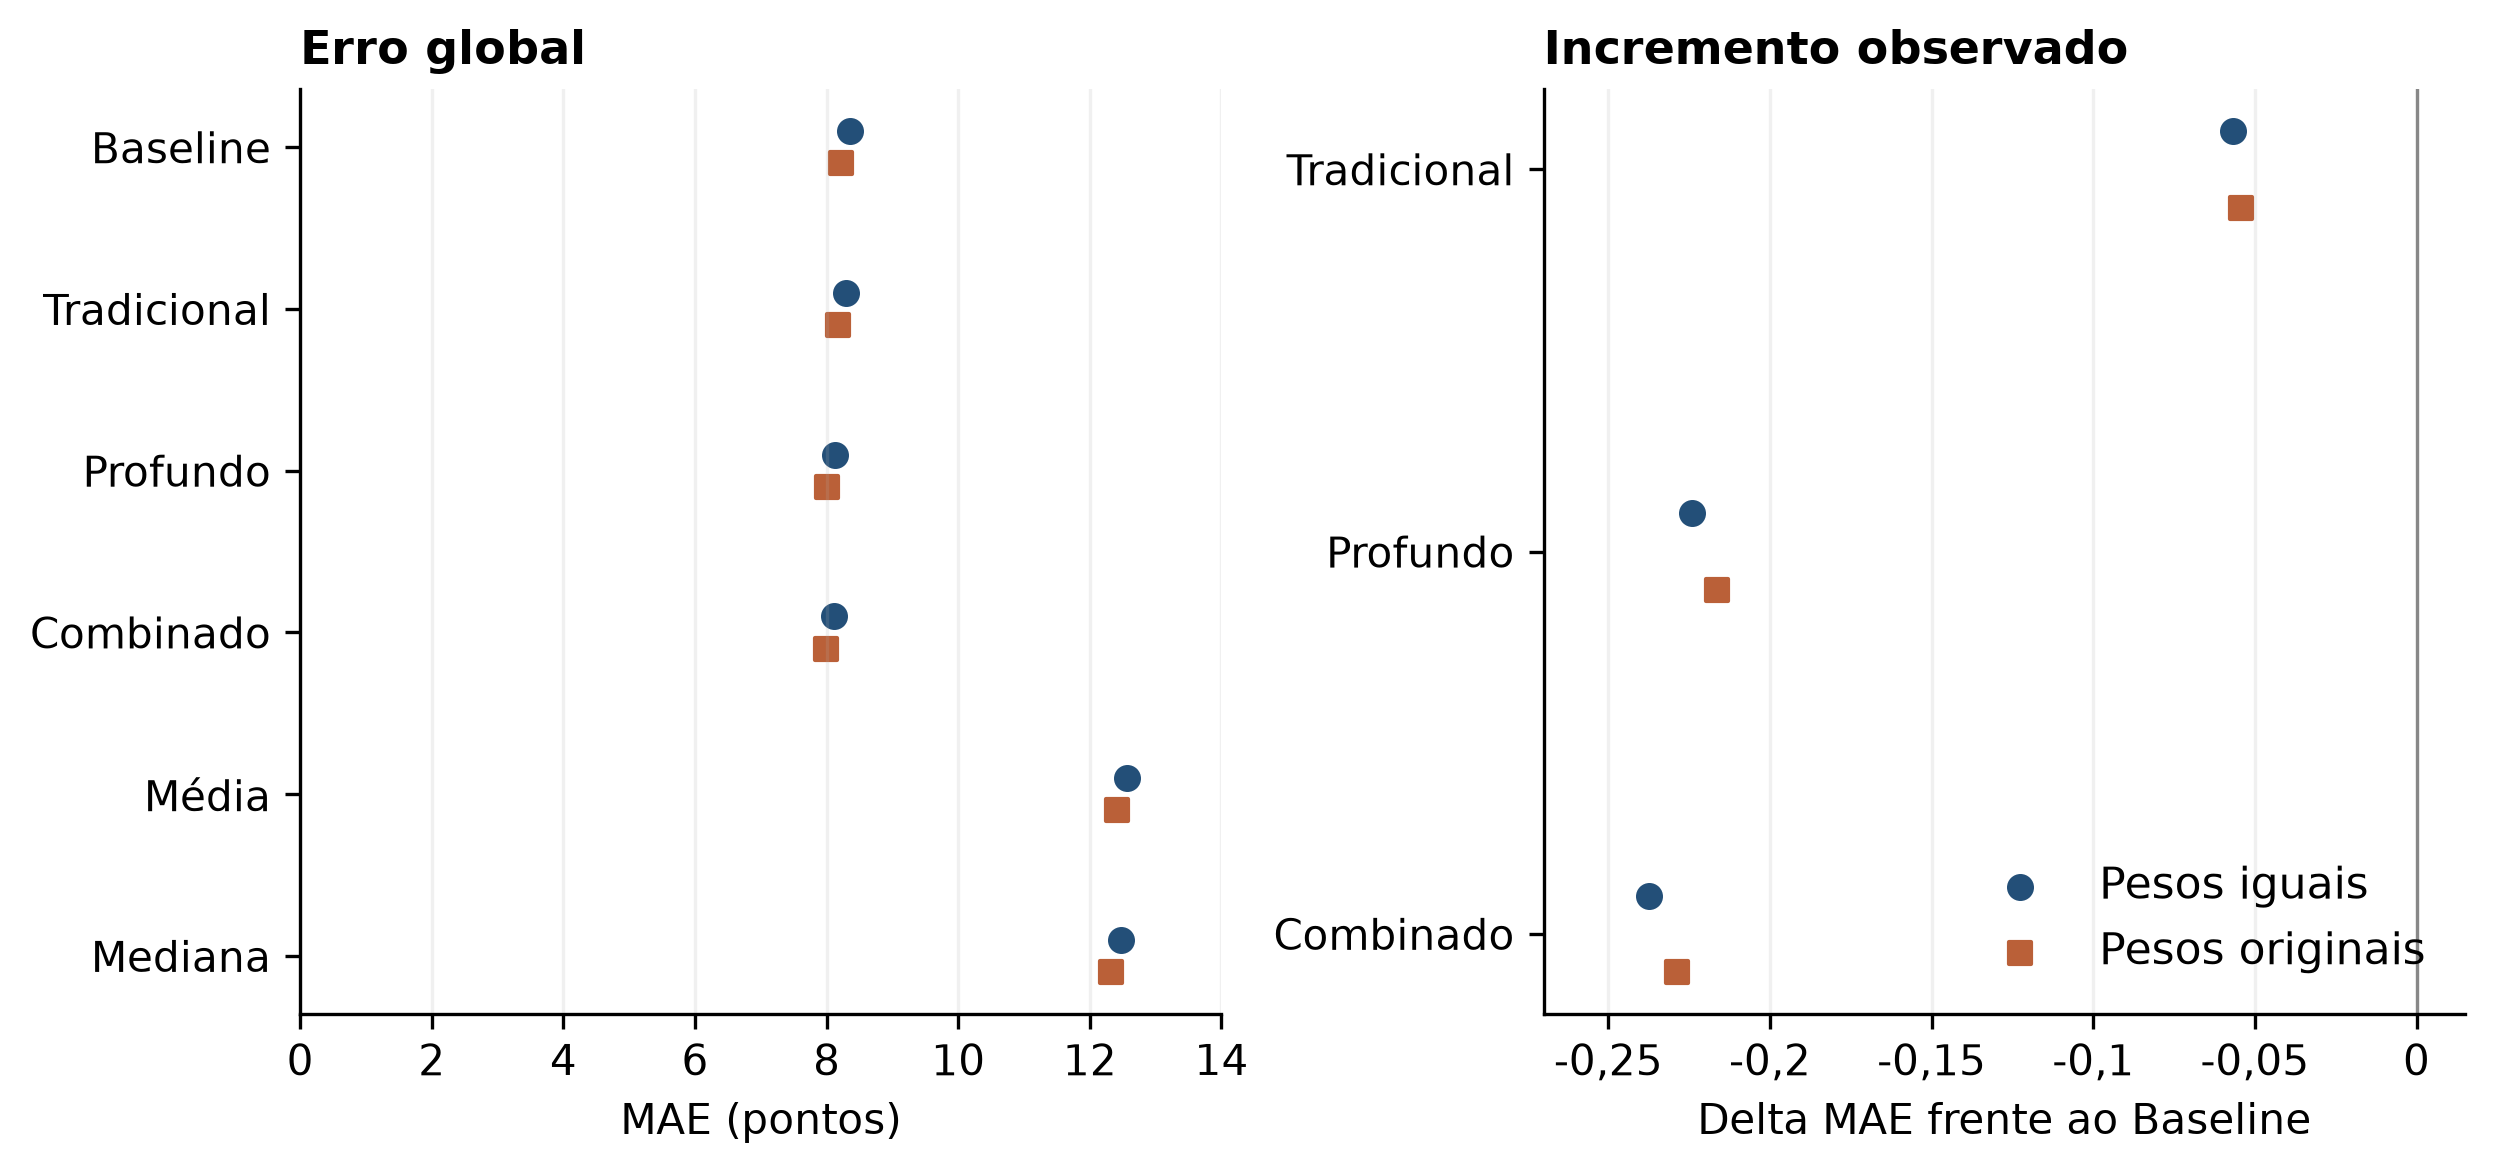
\includegraphics[width=\linewidth]{images/comparacao_global.png}

\caption{MAE global e deltas frente ao Baseline; pontos estimados, sem intervalos de confiança.}

\end{figure}

As referências média e mediana tiveram MAE de 12,5621 e 12,4786. O desempenho melhor das configurações com atributos confirma utilidade preditiva neste procedimento, mas o ganho textual adicional permanece modesto na escala da resposta. Não foi definido um limiar de equivalência prática ou calculado teste de significância.


\FloatBarrier

\clearpage

\section{Estabilidade entre folds e influência dos componentes}

O Combinado teve menor MAE que o Baseline nos cinco folds. Os deltas variaram de -0,2724 a -0,2070. Cada teste externo contém 15.507 faixas; sua estabilidade de direção é descritiva e não autoriza tratar os cinco resultados como réplicas independentes.


\begin{table}[!htbp]\centering\small
\caption{MAE por partição externa.}
\begin{tabularx}{\linewidth}{Xrrrrr}
\toprule
Fold & n & Baseline & Trad. & Prof. & Comb. \\
\midrule
1 & 15.507 & 8,3287 & 8,2526 & 8,1155 & 8,0991 \\
2 & 15.507 & 8,2666 & 8,1989 & 8,0549 & 8,0392 \\
3 & 15.507 & 8,4241 & 8,3673 & 8,2364 & 8,2171 \\
4 & 15.507 & 8,3633 & 8,3211 & 8,1188 & 8,1128 \\
5 & 15.507 & 8,3798 & 8,3385 & 8,1171 & 8,1074 \\
\bottomrule\end{tabularx}
\par\smallskip{\footnotesize Folds numerados de 1 a 5 para apresentação; equivalem aos índices 0 a 4 dos arquivos. Não são réplicas independentes.}
\end{table}


\begin{table}[!htbp]\centering\small
\caption{Influência da retirada de um componente da avaliação.}
\begin{tabularx}{\linewidth}{Xrrr}
\toprule
Contraste & Delta MAE & Mín. remoção & Máx. remoção \\
\midrule
Tradicional - Baseline & -0,0568 & -0,0580 & -0,0557 \\
Profundo - Baseline & -0,2240 & -0,2246 & -0,2225 \\
Combinado - Baseline & -0,2374 & -0,2381 & -0,2359 \\
Combinado - Tradicional & -0,1806 & -0,1814 & -0,1792 \\
Combinado - Profundo & -0,0134 & -0,0138 & -0,0132 \\
\bottomrule\end{tabularx}
\par\smallskip{\footnotesize Modelos e previsões fixos. Estes extremos não são intervalos de confiança, nem validação com retreino.}
\end{table}


\begin{figure}[!htbp]\centering

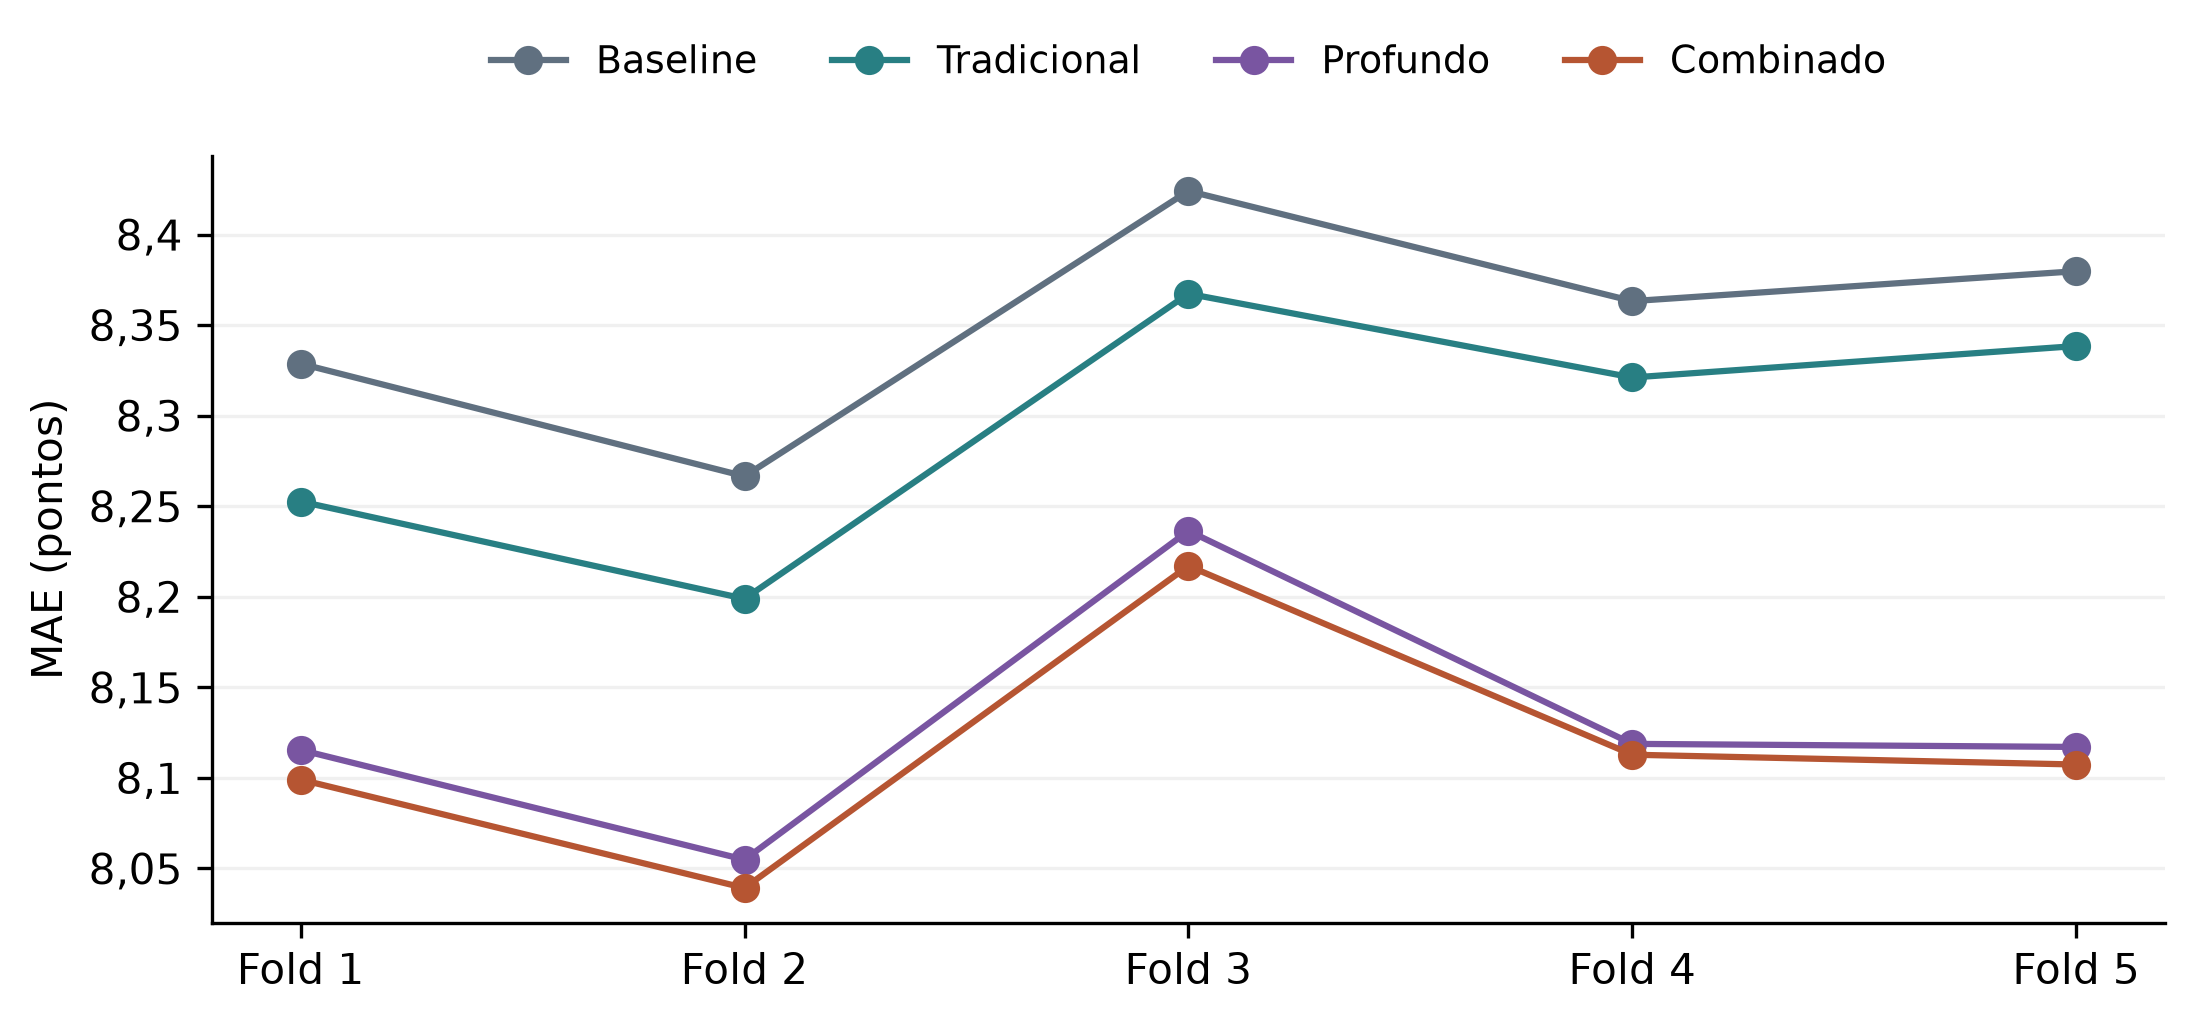
\includegraphics[width=\linewidth]{images/estabilidade_folds.png}

\caption{MAE por fold externo, com as mesmas observações entre blocos em cada partição.}

\end{figure}

Os cinco contrastes mantiveram delta negativo quando qualquer componente foi retirado da avaliação, tanto com pesos iguais quanto com pesos originais. Isso indica que o sinal observado não depende de um único componente avaliado, condicionando aos modelos e previsões fixos. A operação não retreina modelos e não quantifica incerteza do treinamento; seus extremos não são IC.


\FloatBarrier

\clearpage

\section{Erro na cauda de popularidade}

O erro não é uniforme ao longo da resposta. Embora o Combinado melhore o MAE frente ao Baseline em todas as faixas de popularidade publicadas, o erro absoluto cresce na cauda superior. Nas 128 faixas com popularidade entre 80 e 100, o MAE foi 29,3711, contra 30,9294 no Baseline. Esse comportamento deve acompanhar a divulgação do MAE global de 8,1151.


\begin{table}[!htbp]\centering\small
\caption{Erro por faixa de popularidade observada.}
\begin{tabularx}{\linewidth}{Xrrrr}
\toprule
Faixa & n & Baseline & Combinado & Delta MAE \\
\midrule
0-19 & 34.069 & 8,0063 & 7,8177 & -0,1886 \\
20-39 & 30.785 & 6,5204 & 6,4722 & -0,0481 \\
40-59 & 10.968 & 12,2502 & 11,5336 & -0,7165 \\
60-69 & 1.301 & 21,4554 & 19,9204 & -1,5351 \\
70-79 & 284 & 27,7495 & 26,1917 & -1,5578 \\
80-100 & 128 & 30,9294 & 29,3711 & -1,5583 \\
\bottomrule\end{tabularx}
\par\smallskip{\footnotesize Faixas definidas no desenho amostral original. Diagnóstico por resposta observada; não caracteriza desempenho em futuros lançamentos.}
\end{table}


\begin{figure}[!htbp]\centering

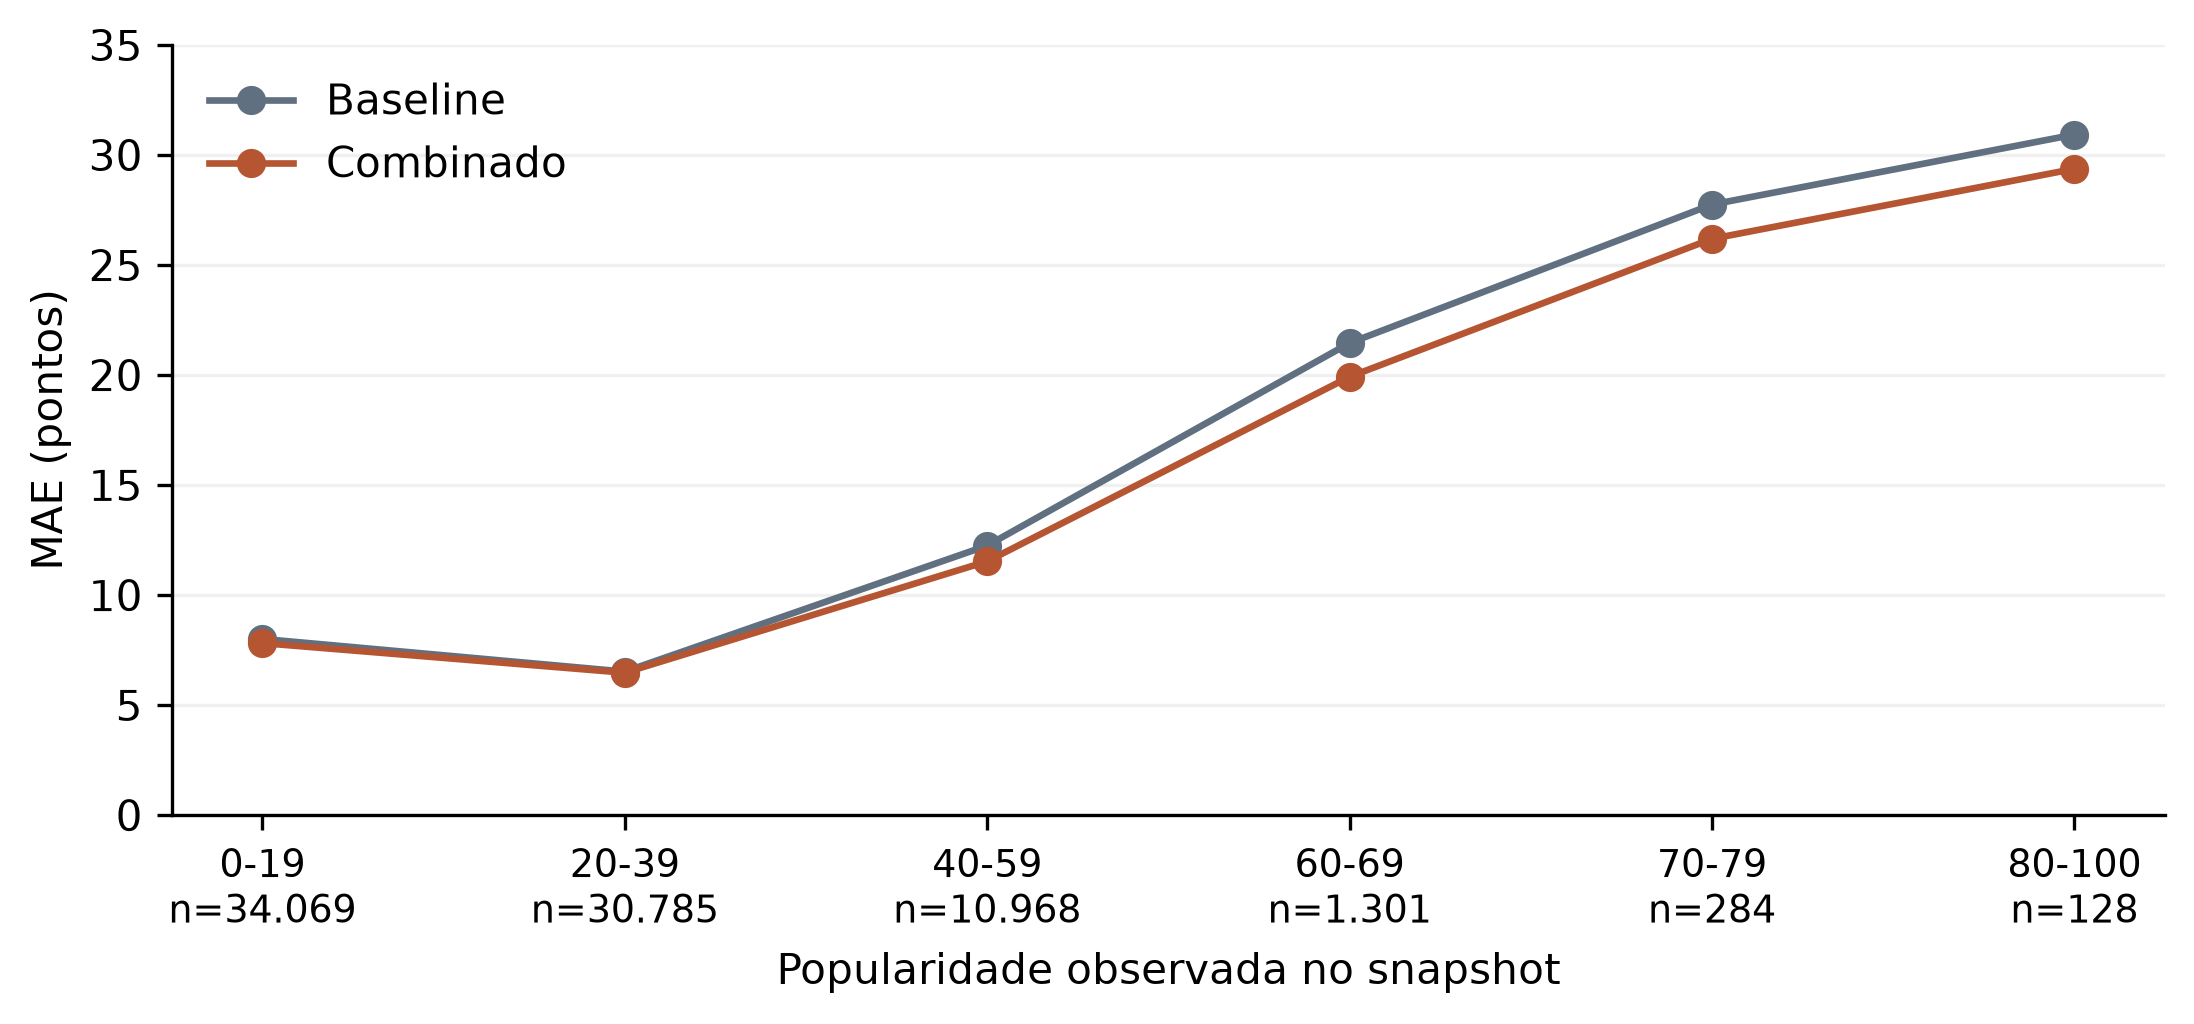
\includegraphics[width=\linewidth]{images/erro_popularidade.png}

\caption{MAE por faixa da resposta observada e número de casos; células pequenas na cauda exigem cautela.}

\end{figure}

As previsões externas máximas do Profundo e do Combinado foram aproximadamente 78 pontos; no Combinado, a mínima foi -32,7066. O protocolo preservou previsões lineares sem clipping: 615 das 77.535 ficaram abaixo de zero. Não se propõe transformá-las retrospectivamente para substituir o resultado principal. Esses diagnósticos não definem um classificador de hits nem avaliação prospectiva de lançamentos.


\FloatBarrier

\clearpage

\section{Heterogeneidade por idioma e outros subgrupos}

O incremento do Combinado frente ao Baseline foi de 0,1561 ponto nas 56.908 faixas de inglês estimado e 0,4693 nas 20.447 classificadas como não inglês. Nas 180 de status incerto, o MAE aumentou de 9,4360 para 9,8564. Portanto, o benefício médio não é uniforme. Essas diferenças descrevem subconjuntos com composição própria, sem identificar um efeito causal do idioma.


\begin{table}[!htbp]\centering\small
\caption{Erro por status de idioma estimado.}
\begin{tabularx}{\linewidth}{Xrrrr}
\toprule
Status & n & Baseline & Combinado & Delta MAE \\
\midrule
Inglês & 56.908 & 7,6840 & 7,5278 & -0,1561 \\
Não inglês & 20.447 & 10,2036 & 9,7343 & -0,4693 \\
Incerto & 180 & 9,4360 & 9,8564 & 0,4204 \\
\bottomrule\end{tabularx}
\par\smallskip{\footnotesize Idioma automático não é verdade humana; subconjuntos diferem também em composição e popularidade. Nenhum idioma foi excluído.}
\end{table}


\begin{figure}[!htbp]\centering

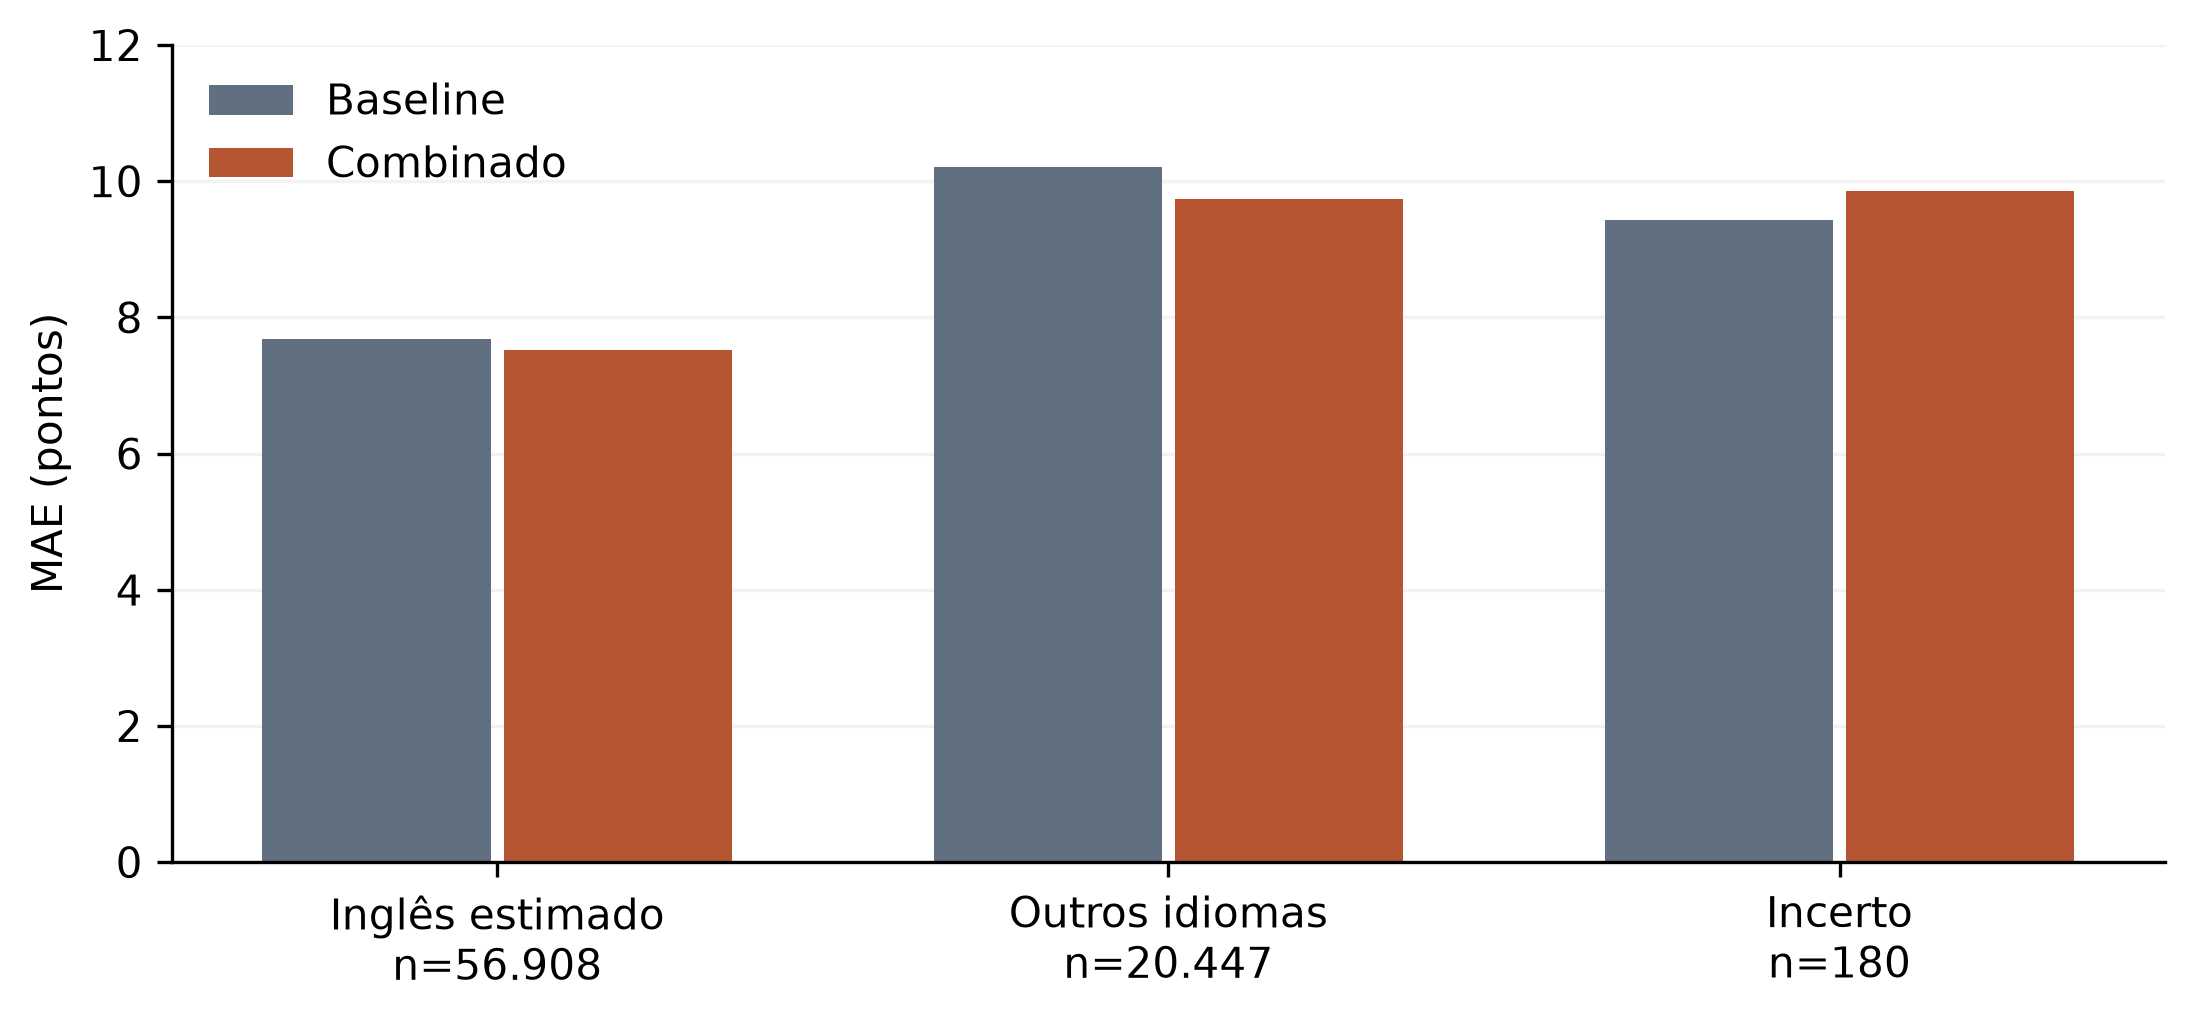
\includegraphics[width=\linewidth]{images/erro_idioma.png}

\caption{MAE por status de idioma automático; o grupo incerto foi mantido na análise principal.}

\end{figure}

Entre os 76 gêneros com métricas publicadas, 59 apresentaram redução do MAE no Combinado frente ao Baseline. Há exceções, e as comparações são exploratórias, sem testes múltiplos. O diagnóstico publicou 116 células e omitiu métricas de 77 células com menos de 100 faixas ou 20 componentes, mantendo apenas suas contagens. Esses limiares não asseguram poder estatístico.


\FloatBarrier

\clearpage

\section{Limites e conclusão descritiva}

O ganho do Combinado também aparece em componentes com colisão histórica detectada e nos sem colisão detectada. Essa separação não constitui novo holdout independente. Os quatro casos de chave histórica indeterminada, pertencentes a um componente, continuam na avaliação global; suas métricas isoladas foram omitidas pelos limiares predefinidos.


A análise sustenta contribuição preditiva incremental observada de letras na comparação Ridge: o bloco de embeddings responde pelo maior incremento, enquanto a adição dos descritores tradicionais a ele produz ganho pequeno. A ordenação global é estável à ponderação e os sinais são preservados nos folds e na retirada condicional de um componente da avaliação.


O alcance permanece limitado ao domínio observado. A integridade técnica não certifica precisão semântica de todos os pares Spotify-LRCLIB; idiomas e identidades são operacionais. As conclusões não são causais, não representam automaticamente o catálogo e não avaliam sucesso comercial futuro. Hipóteses adicionais seriam necessárias para ampliar a inferência.


Não foram calculados IC ou p-valores. Bengio e Grandvalet (2004) mostram por que ignorar correlações na CV pode subestimar a variância. Os resultados apresentados não estabelecem significância estatística. Qualquer análise inferencial adicional deverá declarar seu estimando, hipóteses e tratamento da dependência dos ajustes.


\begin{table}[!htbp]\centering\small
\caption{Diagnóstico de colisão com avaliação histórica por componente.}
\begin{tabularx}{\linewidth}{Xrrr}
\toprule
Status histórico & n & Baseline & Combinado \\
\midrule
Colisão detectada & 7.170 & 7,7635 & 7,5606 \\
Sem detecção & 70.361 & 8,4126 & 8,1716 \\
Chave indeterminada & 4 & omitido & omitido \\
\bottomrule\end{tabularx}
\par\smallskip{\footnotesize Quatro casos de um componente permanecem no resultado global. Ausência de colisão detectada não garante independência histórica.}
\end{table}


Esta consolidação é um trecho parcial de métodos, resultados e discussão para a monografia. Não substitui introdução, revisão bibliográfica, caracterização completa das fontes, revisão dirigida de matching ou adequação ao template institucional. Os dados, modelos, pesos e folds anteriores permanecem preservados.


\FloatBarrier
